\documentclass[11pt, a4paper]{article}
\usepackage[T2A]{fontenc}
\usepackage[utf8]{inputenc}
\usepackage[bulgarian]{babel}

%% Sets page size and margins
\usepackage[a4paper,top=3cm,bottom=3cm,left=3cm,right=3cm,marginparwidth=1.75cm]{geometry}

%% Useful packages
\usepackage{amsmath, amssymb, amsthm,calc,mathabx}
\usepackage{systeme}
\usepackage{graphicx}
\usepackage[colorinlistoftodos]{todonotes}
\usepackage[colorlinks=true, allcolors=black]{hyperref}
\usepackage{wrapfig,lipsum,booktabs}
\usepackage{enumitem}
\usepackage{float}
\usepackage{fmtcount}
\usepackage{multicol}
\usepackage{breqn}
\usepackage{setspace}
\usepackage{hyperref}
\usepackage {tikz}
	\usetikzlibrary {positioning}
	
\graphicspath{
	{Graphics/}
}

\newtheorem{theorem}{Theorem}

\newtheorem{lemma}{Lemma}
\newtheorem{prop}{Property}
\newtheorem*{remark}{Remark}

\theoremstyle{definition}
\newtheorem{definition}{Дефиниция}

\setlength{\columnsep}{1cm}
\setlength{\parindent}{1em}

\begin{document}
\begin{titlepage}
	\newcommand{\HRule}{\rule{\linewidth}{0.5mm}}
	\centering
	\textsc{\LARGE SRS 2019}\\[1cm]
	\HRule\\[1 cm]
	
	{\huge\bfseries Рансъмуер Research Project }\\[0.5 cm] 
	\HRule\\
    \vfill
			\Large
			\textit{Автор:}
			 \textsc{Nikola Staykov}\\
             \vspace{2cm}
			\Large
			\textit{Ментор:}
            \textsc{Явор Папазов}
    \vfill	
	{\large\today}   
	\vfill
\end{titlepage}

\tableofcontents
\newpage
\begin{abstract}
		Рансъмуер е вид компютърен вирус, който критптира файловете на дадена система и изисква да бъде платен откуп, за да бъдат декриптирани. Приемаме, че създателите на рансъмуер не знаят цената на данните на техните жертви, или по-точно колко техните жертви $\dq \text{мислят} \dq$ , че струват данните им. Те могат да правят малки проучвания преди да започнат основната кампания с цел да определят гореспоменатото разпределение. Този проект разглежда модел, чрез който да бъдат определени оптималните параметри за едно такова проучване. Този подход е ключов за намирането на оптималната цена за откупа.
\end{abstract}

\section{Въведение}
		Рансъмуер се появява за първи път през 1989 под формата на the AIDS Troyan, познат също като PC Cyborg.  The AIDS Trojan е бил доста лесен за преодоляване, тъй като използва симетрична криптография, и скоро са били разработени начини файловете да бъдат декриптирани, но този случай поставя началото на развитието на много от модерните заплахи. С навлизането на Интернет, рансъмуер се завръща с нова сили, а именно с the Archiveus Trojan и GPcode от 2006. Друг повратен момент в историята на рансъмуер е създаването на биткойн, и крипто-валутите като цяло, по много причини, някои от тях бидейки анонимността и автоматичните и невъзвръщаеми транзакции\cite{huang2018tracking}.\par
		В изминалите години е имало опити да бъде направен модел на пазара на malware. В \cite{caulfielddynamic}, авторите са създали теоретичен модел, взимайки предвид броя потребители, които имат бекъпи, както и други фактори като разпространението на информация и надеждност на рансъмуер.           
		В \cite{cartwright2018pay} е изследван различен подход, който разглежда възможността за допълнително уговаряне на цената като игра между жертвата и престъпниците. Тази разработка се фокусира на теория на игрите и комбинаторика.\par
		Доста усилия са положени и за проследяването на плащания, свързани с рансъмуер в блокчейн, тъй като всички те са публични. В резултат на това има публични данни, свързани с тези плащания, предоставени от \cite{paquet2019ransomware} и в \cite{thomas2015framing} човек може да се запознае с много заключенияв, подкрепени с данни, отнасящи се не само до рансъмуер, но и до целия черен пазар.\par
		Моделът в настоящата разработка е базиран на описания в \cite{caulfielddynamic}, но се фокусира върху оптимизирането на параметри, които не са разгледани в споменатата статия.
\newpage
	\section{Теория}
	В тази секция са включени всички дефиниции и концепции, които са нужни за цялостното разбиране на проекта.
		\begin{definition}
			\label{def:normdist}
			\emph{Нормално разпределение}, означено  с $N(\mu, \sigma)$, е вид непрекъснато разпределение, където с $\mu$, $\sigma$ и $\sigma^{2}$ са означени среднoто аритметично, стандартната девиация и вариацията съответно.
		\end{definition}
	
		Графиката на тази функция образува крива, често наричана също камбанна крива. Тя има максимум $(x,f(x))$ в $\left(\mu, \dfrac{1}{\sigma\sqrt{2\pi}}\right)$:
		\begin{center}
			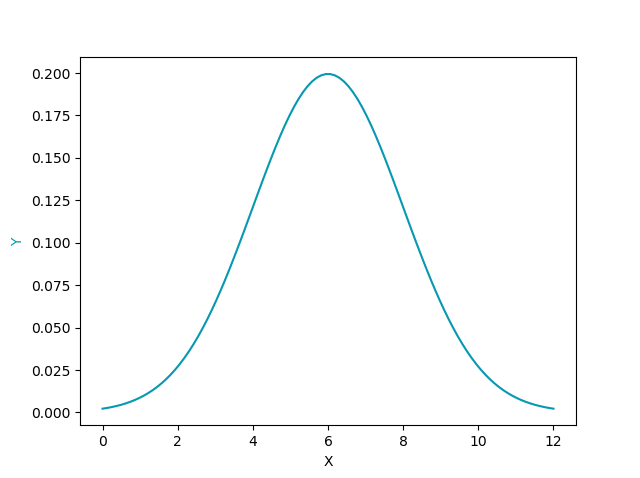
\includegraphics[width=0.6\textwidth]{Normal_clean}
		\end{center}
		
		\begin{definition}
			\label{def:def2}
			Разглеждаме нормално разпределение $N(\mu, \sigma)$. \emph{Стандартната стойност}, или \emph{Z-score}, на дадено $x$ показва колко стандартни девиации е то от дадената средна стойност. Пресмята се по формулата $\dfrac{x-\mu}{\sigma}$.
		\end{definition}
	
		\begin{definition}
			\label{def:prob_dist}
			За дадено разпределение \emph{функцията на разпределение} $F(x)$ показва вероятността стохастична променлива, следваща разпределението, да е по-малка или равна на $x$
			$$F_{X}(x)=\mathbb{P}(x\leq X).$$
		\end{definition}
	
		\begin{definition}
			\label{def:prob_dens}
			\emph{Плътност на разпределение} на непрекъсната стохастична променлива $x$, описва вероятността дадена стохастична променлива $x$ да се окаже в произволен интервал. Формално се дефинира чрез
			\begin{align*}
				&\mathbb{P}(x < X \leq x+\Delta)=F_X(x+\Delta)-F_X(x)\\
				&f_X(x)=\lim_{\Delta \rightarrow 0} \frac{F_X(x+\Delta)-F_X(x)}{\Delta}.		
			\end{align*}
		\end{definition}
	
		\begin{definition}
			\label{def:err}
			\emph{Грешка от първи род} е резултат на интегрирането на нормално разпределение, тя приема z-score като параметър и пресмята интеграла между фиксирана точка и средната стойност за разпределението.
			$$\operatorname{erf}(z)=\dfrac{2}{\sqrt{\pi}}\int_{0}^{z}e^{-t^{2}}dt.$$
		\end{definition}
	
	\section{Подход}
		Този модел описва разпространението на рансъмуер вирус. Намира оптималната цена на откуп за рансъмуер атака, която използва единствено botnets, без ключовия компонент на разпространяване на всеки компютър в мрежата. Този вариант на атаката е сравнително евтин за осъществяване, но има ниска ефективност. Третираме декриптирането на файловете на даден компютър като услуга, а откупа като нейната цена, съответно. \par
		Разглеждаме разпределението на Желанието за плащане (ЖЗП) на дадена тестова група. Това е максималната сума, която някой би платил за данните си. Поставяйки се в позицията на престъпниците се опитваме да открием разпределението чрез изследването на тестови групи от хора и как те реагират на дадена цена. Тези тестове обаче ни струват ценно време тъй като осведомеността на хората се показва постоянно. Искаме да разберем колко и колко големи тестове трябва да провеждаме, така че да направим модел на разпределението с приемлива грешка и в същото време без да губим твърде много време.\par
		За даден размер на тестовата група, изчисляваме грешката на дадена група от "потребители" от математически описаната функция на кривата на търсенето, която извличаме от разпределението на ЖЗП. Започвайки с малка група, постепенно увеличаваме размера на тестовата група, изчислявайки и грешката чрез метода на най-малките квадрати на всяка стъпка.
	\section{Модел}
		Тук математическата страна на модела е разгледана подробно, показвайки как са достигнати резултатите и закюченията. Секцията е разделена на две смислови части, съответстващи на параметрите, които моделът изследва.
		\subsection{Размер на тестовата група и грешка}
			Тази секция описва математическия модел, използвам за оптимизиране на грешката. Изведени са заключения относно размера на тестовата група.\par
			Приемаме, че стойността на данните на хората следва нормална дистрибуция и я свързваме със стохастичната променлива $p\sim N(500, 150)$. Вероятностната плътност (ВП) на нормална дистрибуция $N(\mu, \sigma)$ е $$\frac{1}{\sigma\sqrt{2\pi}}e^{-\frac{(x-\mu)^{2}}{2\sigma^{2}}}.$$\par\noindent
			За да изчислим функцията на търсене $f(k)$ от ВП за дадена цена $k$, трябва да изчислим
			$$\int_{k}^{\infty}f(x)\operatorname{d} x.$$
			\begin{figure}[H]
				\begin{minipage}{0.48\textwidth}
					\centering
					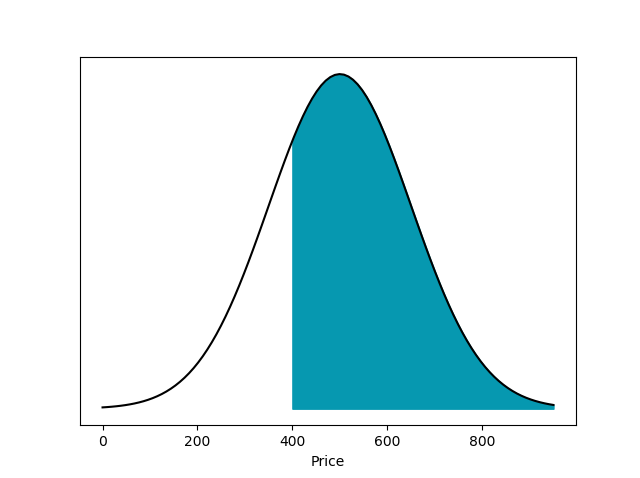
\includegraphics[width=\linewidth]{ND_integral}
					\caption{ВП}\label{Fig:Data1}
				\end{minipage}$\longrightarrow$
				\begin{minipage}{0.48\textwidth}
					\centering
					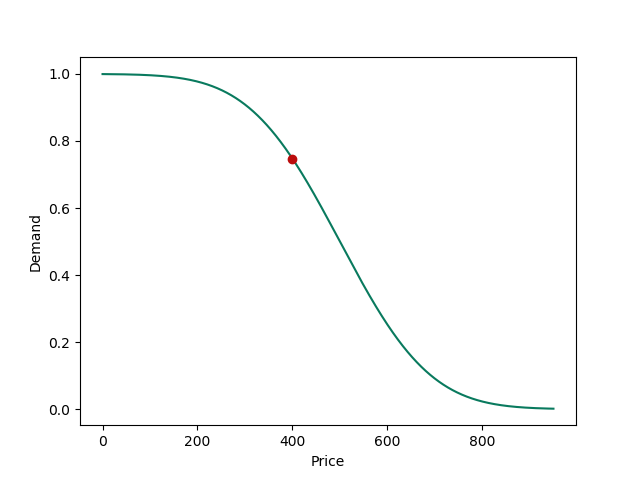
\includegraphics[width=\linewidth]{Sample_point}
					\caption{Цена и търсене}\label{Fig:Data2}
				\end{minipage}
			\end{figure}\par\noindent
			Отбелязаме, че интегралът трябва да бъде изчилсен до безкрайност, но след като $k$ стигне $\mu+3\sigma$, резултатът става пренебрежимо малък. Правейки това за цялата функция на разпределението получаваме кривата на търсенето чрез процента хора, които биха платили. Нека означим кривата на търсенето с $F(x)$:
			$$
			F(x)=
			\begin{cases}
				\dfrac{1}{2}\left (1-\operatorname{erf}\left (\dfrac{z}{\sqrt{2}}\right )\right ) \text{ако } x>\mu,\\
				\\
				\dfrac{1}{2}\left (1+\operatorname{erf}\left (\dfrac{z}{\sqrt{2}}\right )\right ) \text{ако } x<\mu.
			\end{cases}
			$$\par
			Искаме да оптимизираме броя хора във всяка тестова група. Математическата функция, която искаме да опишем ни дава възможността да изчислим грешките от експерименталните данни с максимална точност.
			\begin{figure}[H]
				\begin{minipage}{0.48\textwidth}
					\centering
					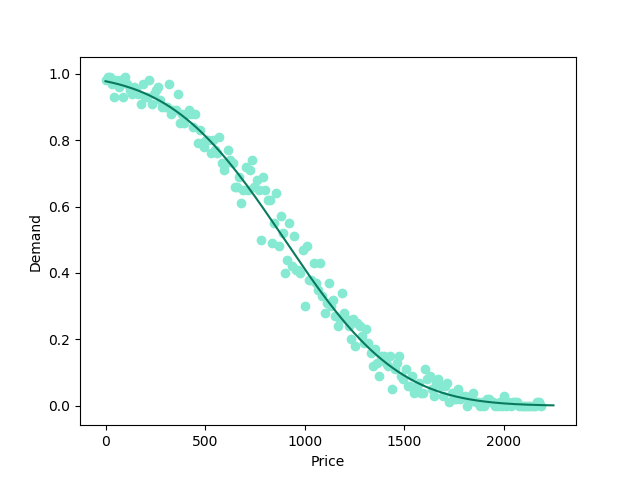
\includegraphics[width=\linewidth]{Exp_and_math_100}
					\caption{100 човека в групата}\label{Fig:Data3}
				\end{minipage}\hfill
				\begin{minipage}{0.48\textwidth}
					\centering
					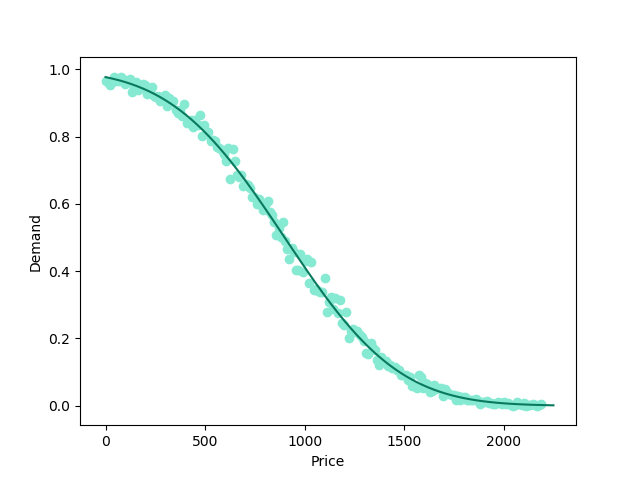
\includegraphics[width=\linewidth]{Exp_and_math_400}
					\caption{400 човека в групата}\label{Fig:Data4}
				\end{minipage}
			\end{figure}\par\noindent
			Събирайки информация за размера на тестовата груап и грешките, съставяме графика, която показва тези промени.
			\begin{figure}[H]
			\begin{minipage}{1.0\textwidth}
				\centering
				\includegraphics[width=0.7\textwidth]{\dq Error vs sample size 4\dq}
				\caption{Тестов размер и грешка}\label{Fig:Data5}
			\end{minipage}
			\end{figure}
		\subsection{Бекъп функция}
			В тази секция описваме функция, отговаряща за вероятността за присъствието на бекъп. Изчислен е ефектът и върху очакваната печалба.\par
			Първо нека дефинираме бекъп итератора $b$: 
			$$
			b=
			\begin{cases}
				1 \text{ ако жертвата има бекъп},\\
				0 \text{ ако жертвата няма бекъп}
			\end{cases}
			$$
			Сега нека дефинираме желанието за плащане (ЖЗП):
			$$
			P(x)=
			\begin{cases}
			d_{x} \text{ ако } b_{i}=0,\\
			c \text{ ако } b_{i}=1
			\end{cases}
			$$
			Тук цената на бекъп е означена с $c$, а цената на данните на жертвата- с $d_{x}$.\par
			Както и по-рано, изчисляваме очакваната вероятност даден човек да плати цена $x$.
			Приемаме, че вероятността конкретна жертва да има бекъп е константа $p$ и изследваме как промяната на тази стойност влияе на очакваната печалба. Чрез събраните данни създаваме графика, която показва връзката между двете променливи. Измерената грешка е относителна.
			\begin{center}
				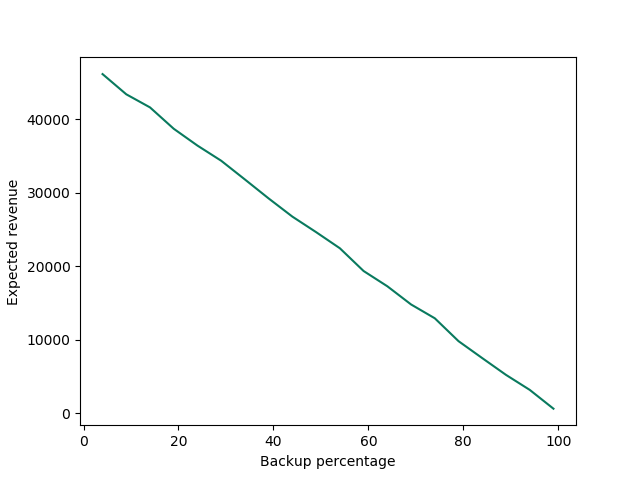
\includegraphics[width=0.55\textwidth]{Revenue_vs_backup}
			\end{center}
			
\section{Резултати}
	Изследвахме как размерът на тестовата група влияе на грешката на експерименталните данни и също как процента на защитените с бекъпи влияе на очакваната печалба. Моделът се фокусира на оптимизирането на цената на откупа, но авторът вярва, че за да можем да предприемем подходящи предпазни мерки срещу атаки от този вид, трябва да разбираме всеки ход на престъпниците. Поставяйки се на мястото на извършителите е ключово за целта. Допълнителни резултати, като връзката между очакваната печалба и броя на хората с бекъпи може да ни помогне да стигнем до подходящи подходи за справяне със заплахата.
\section{Бъдещо развитие}
	Авторът предвижда бъдещето развитие а проекта в няколко посоки, а именно:
	\begin{itemize}
		\item търсене на връзка между бекъпите и ЖЗП разпеделението
		\item разширяване на модела с цел да описва по-сложен начин на разпространение между машините в дадена система
		\item използването на разултатите и данните на други подобни разработки с цел подкрепянето на проекта с реални данни\cite{paquet2019ransomware}
		\item разглеждане на динамичен модел за определяне на цената.
	\end{itemize}
\section{Благодарности}
Искам да благодаря на своя ментор, Явор Папазов, и на Константин Делчев за безотказната помощ в избора на темата на проекта и последващото му развитие, за снабдяването ми с всички нужни материали за запознаването ми с темата, както и за изслушването на въпросите ми. Искам също да благодаря на Станислав Харизанов за професионалните съвети.
\nocite{*}
\bibliographystyle{unsrt}
\bibliography{Bibliography}
\end{document}